\input ../SlidePreamble
\input ../preamble


\begin{document}

{\Huge

  \centerline{\bf TTIC 31230, Fundamentals of Deep Learning}
  \bigskip
  \centerline{David McAllester, Autumn 2021}
  \vfill
  \vfil
  \centerline{Vector Quantized Variational Autoencoders (VQ-VAEs)}
  \vfill
  \vfill

\slide{Gaussian VAEs for Faces 2014}

We can sample faces from the VAE by sampling noise $z$ from $p_\pri(z)$ and then sampling an image $y$ from $p_\dec(y|z)$.

\vfill
\centerline{\includegraphics[width = 3in]{\images/VariationalFaces}}
\centerline{[Alec Radford]}

\slide{VQ-VAEs 2019}

\centerline{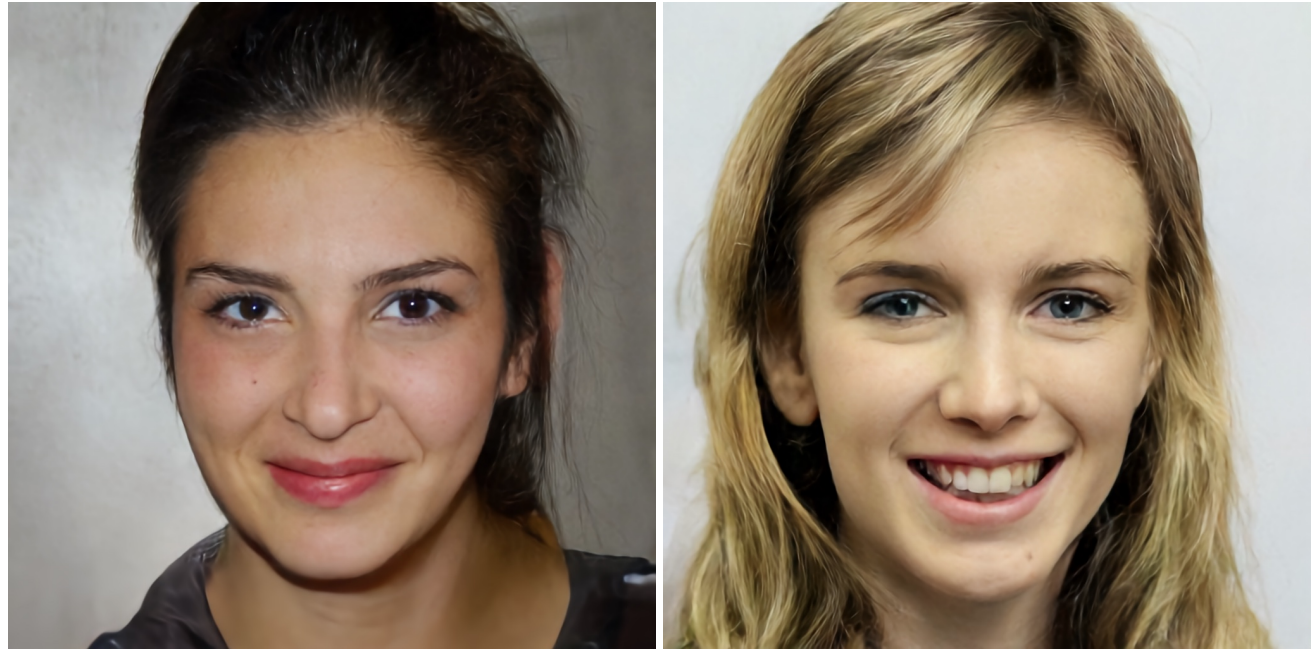
\includegraphics[width = 8in]{\images/VQ-VAE22}}

\vfill
VQ-VAE-2, Razavi et al. June, 2019

\slide{VQ-VAEs 2019}

\centerline{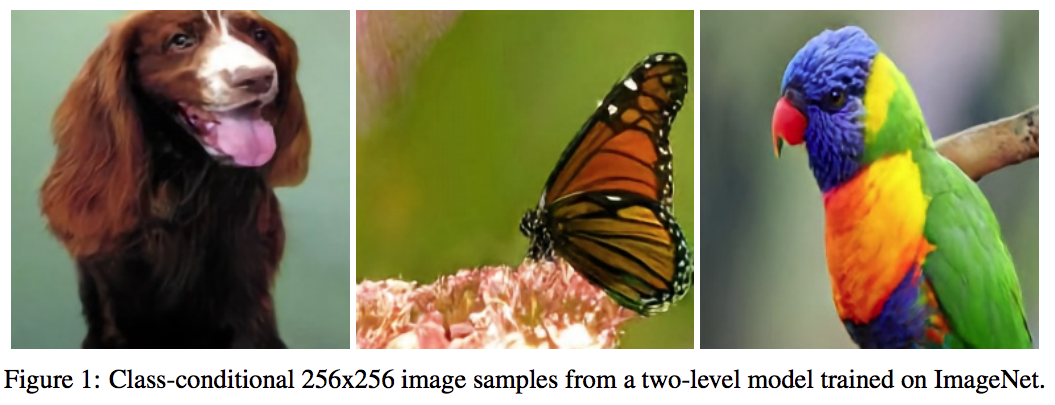
\includegraphics[width = 10in]{\images/VQ-VAE21}}

\vfill
VQ-VAE-2, Razavi et al. June, 2019



\slide{VQ-VAE-2 Model}


\centerline{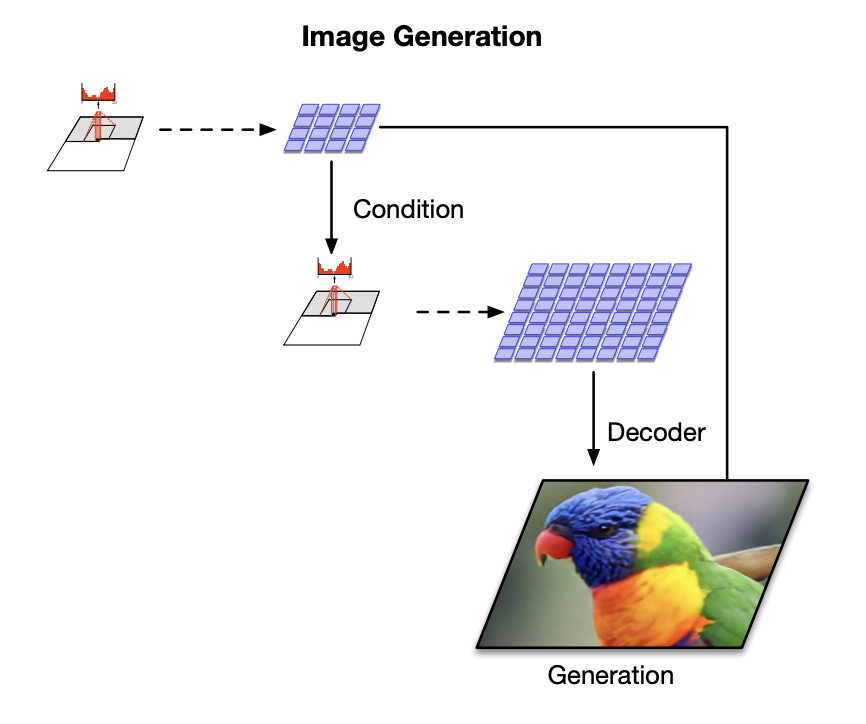
\includegraphics[height =2in]{\images/VQSampler}}

\vfill
The probability of an image $y$ is defined by the generator.

\vfill
The generator is top-down and is similar to that of a progressive GAN.


\slide{VQ-VAE-2 Model}

We describe the case of just one layer.

\vfill
\centerline{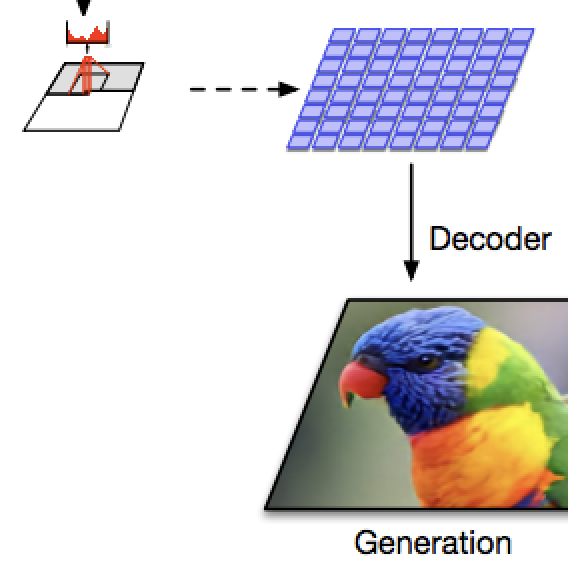
\includegraphics[height = 2in]{\images/VQ-OneLayer}}

\vfill
A separate unit describes progressive VAEs which are inspired by an analogy with progressive GANs.  Progressive VAEs provide a speculative method
of multi-layer VQ-VAE training.

\slide{The Encoder}

Let $s$ denote the image (we are using $y$ for an image coordinate).

\vfill
We have an encoder network, such as a CNN, which produces a layer $L_\enc(s)[X,Y,I]$ with a vector at each pixel position.

\vfill
Intuitively we cluster the vectors $L_\enc(s)[x,y,I]$ using K-means clustering to produce cluster centers where $C[k,I]$
is the cluster center vector of cluster $k$.

\vfill
The set of cluster centers $C[K,I]$ is a trained parameter of the encoder.

\slide{The Encoder}

We then find the nearest cluster center to each vector $L_\enc(s)[x,y,I]$.

\vfill
$$k_\enc(s)[x,y] = \argmin_k \;||L_\enc(s)[x,y,I] - C[k,I]||$$

\vfill
The ``symbolic image'' $k_\enc(s)[X,Y]$ is the latent variable $z$.

\slide{The Decoder}

To decode $z$ we first construct a layer using the cluster center vectors at each $x,y$ position.

$$\hat{L}_\dec(z)[x,y,I] = C[k[x,y],I]$$

\vfill
Finally we decode $\hat{L}_\dec(z)[X,Y,I]$ to get an image $\hat{s}_\dec(z)$.

\slide{Two-Phase Optimization}

{\huge
{\bf Phase 1:} Train the encoder and the decoder to minimize reconstruction error.

$$\enc^*,\dec^* = \argmin_{\enc,\dec}\;E_{s \sim \pop,z \sim P_\enc(z|s)}\left[-\ln P_\dec(s|z)\right]$$


\vfill
{\bf Phase 2:} Train the prior holding the encoder and decoder fixed.

$$\pri^*   =  \argmin_{\pri}\;E_{s\sim \pop,z\sim P_\enc(z|s)}\left[-\ln P_\pri(z)\right]$$

\vfill
Under the universality assumption this two phase method succeeds in modeling the popluation ---
for any encoder it suffices to optimize the decoder and the prior.


\slide{Image Autoencoding}

The VQ-VAE for images uses

\vfill
$$\enc^*,\dec^* = \argmin_{\enc,\dec}\;E_{s \sim \pop}\left[||s - \hat{s}_\dec(z_\enc(s))||^2\right]$$

\slide{Handling Discrete Latents}

$$\enc^*,\dec^* = \argmin_{\enc,\dec}\;E_{s \sim \pop}\left[||s - \hat{s}_\dec(z_\enc(s))||^2\right]$$

\vfill
Since $z = k_\enc(s)[x,y]$ is discrete we have

\vfill
$$k_\enc(s)[x,y].\grad = 0.$$

\slide{Handling Discrete Latents}

$$\enc^*,\dec^* = \argmin_{\enc,\dec}\;E_{s \sim \pop}\left[||s - \hat{s}_\dec(z_\enc(s))||^2\right]$$

\vfill
VQ-VAE uses ``straight-through'' gradients and ``k-means'' gradients.

{\huge
\begin{eqnarray*}
L_\enc(s)[x,y,I].\grad & = & \hat{L}_\dec(z)[x,y,I].\grad + \beta(L_\enc(s)[x,y,I] - C[k_\enc(s)[x,y],I]) \\
\\
C[k,I].\grad & = & \sum_{k_\enc(s)[x,y]=k} \gamma(C[k,I] - L_\enc(s)[x,y,I])
\end{eqnarray*}
}

\slide{One Layer VQ-VAE Training Phase 2}

Finally we hold the encoder fixed and train the prior $P_\pri(z)$ to be an auto-regressive model of the symbolic image $k_\enc(s)[X,Y]$.

\vfill
\centerline{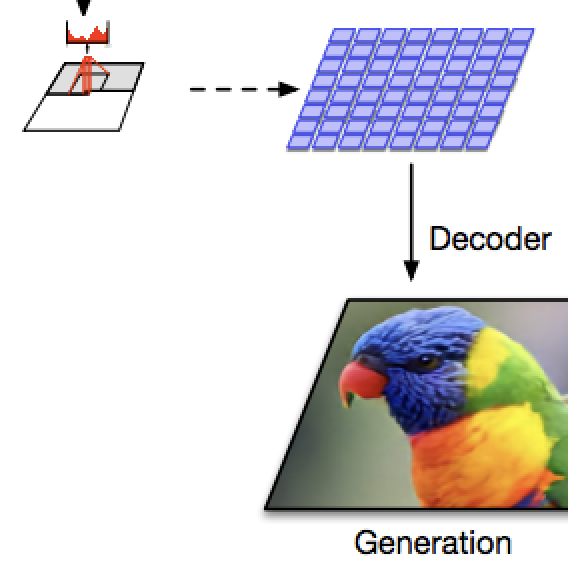
\includegraphics[height = 2in]{\images/VQ-OneLayer}}

\slide{Quantitative Evaluation}

The VQ-VAE2 paper reports a classification accuracy score (CAS) for class-conditional image generation.

\vfill
We generate image-class pairs from the generative model trained on the ImageNet training data.

\vfill
We then train an image classifier from the generated pairs and measure its accuracy on the ImageNet test set.

\vfill
\centerline{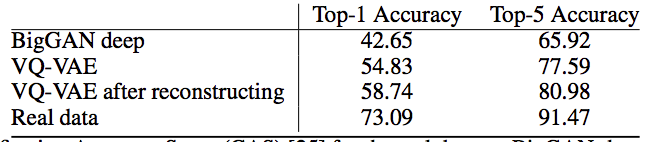
\includegraphics[width=7in]{\images/VQ-VAE23}}

\slide{Image Compression}

\vfill
\centerline{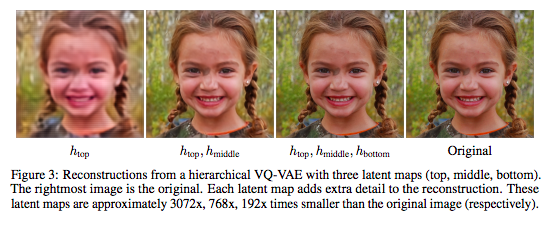
\includegraphics[width = 10in]{\images/VQgirl}}

\slide{Rate-Distortion Evaluation.}

Rate-distortion metrics for image compression to discrete representations support unambiguous rate-distortion evaluation.

\vfill
Rate-distortion metrics also allow one to explore the rate-distortion trade-off.

\vfill
\centerline{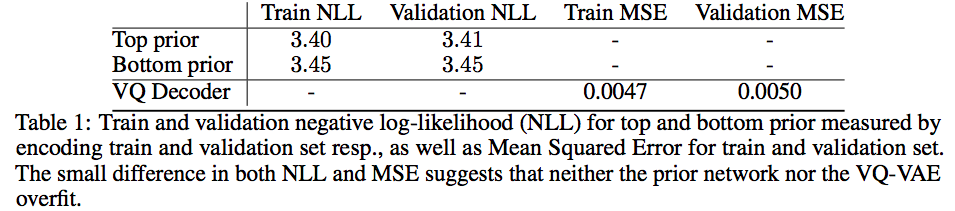
\includegraphics[width = 10in]{\images/VQVAE2Scores}}

\slide{DALL$\cdot$E: A Text-Conditional Image dVAE}
\vfill
DALL$\cdot$E is a text-conditional VQ-VAE model of images.

\vfill
The Vector quantization is done independent of the text.  However, the model of the probability distribution of the symbolic image $z[x,y]$ is conditioned on text.

\vfill
\centerline{\huge Ramesh et al. 2021}


\slide{DALL$\cdot$E}

\centerline{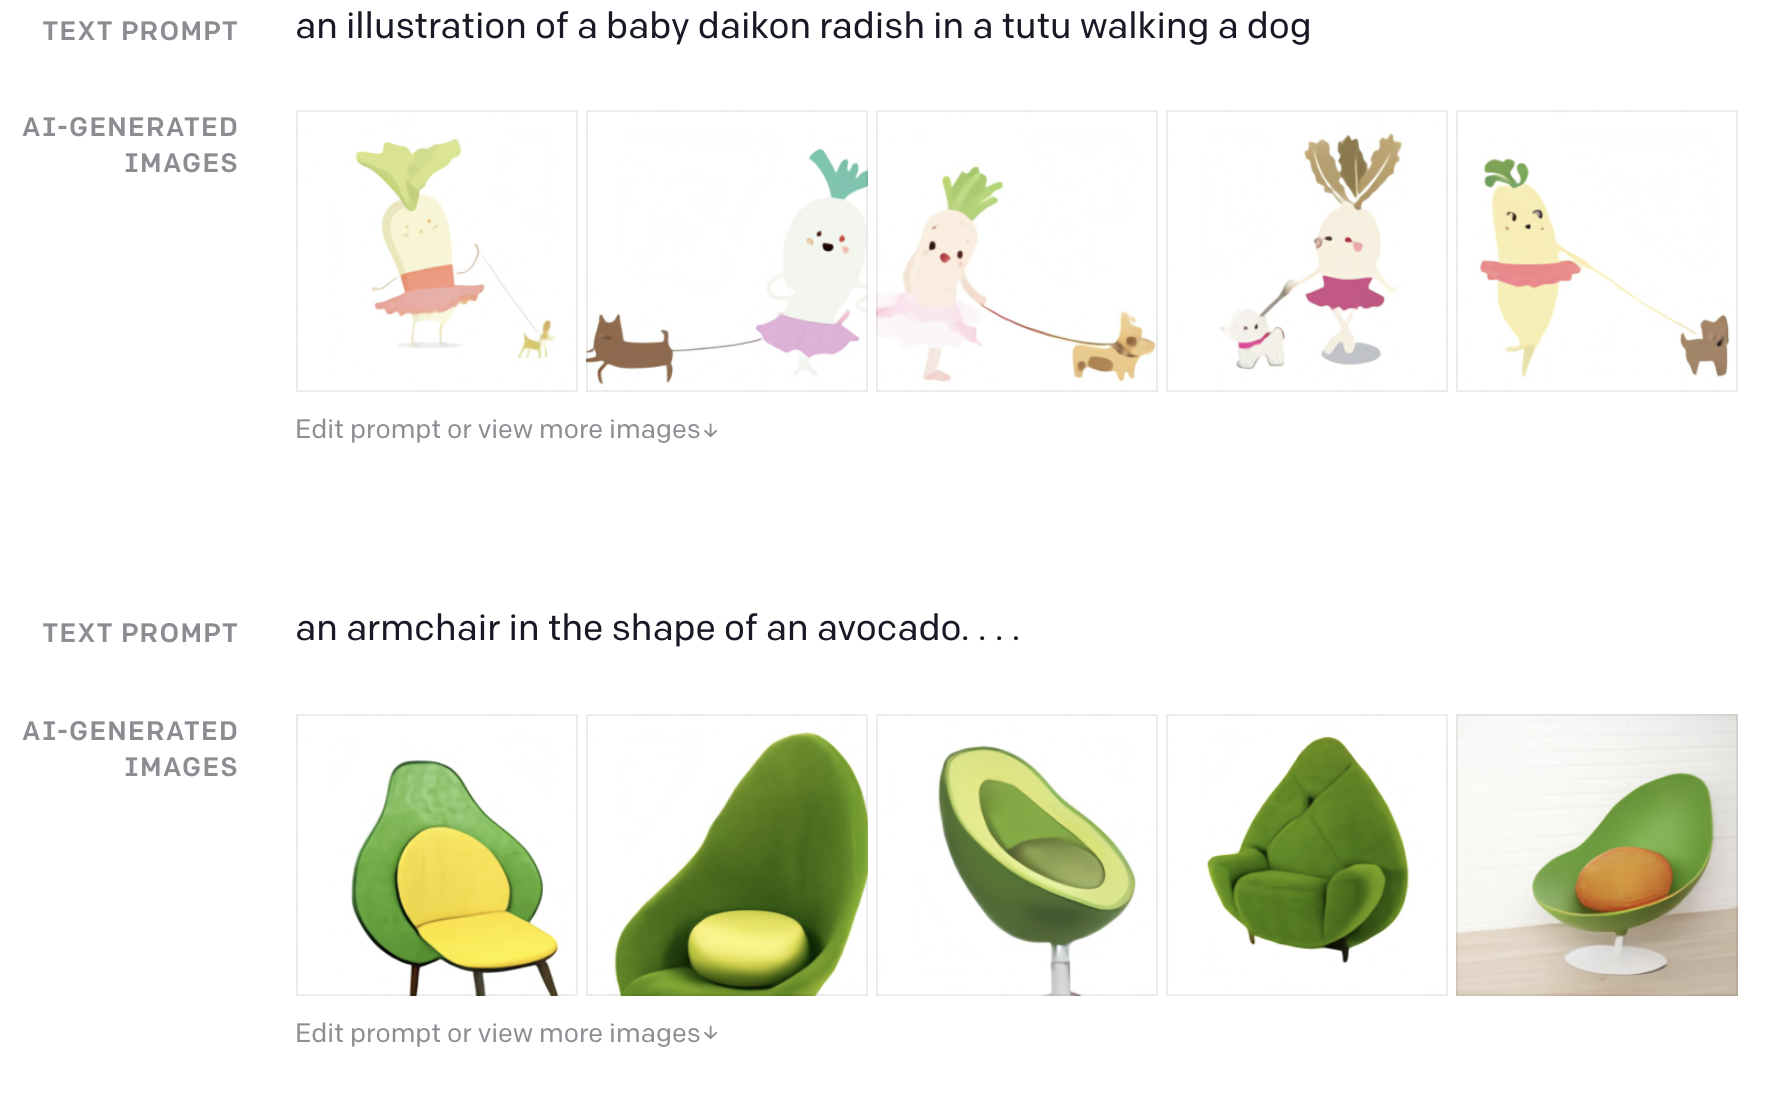
\includegraphics[height= 5.5in]{\images/DALLE1}}

\slideplain{END}

\end{document}
